\section{Odd One Out Learning}\label{sec:o3n}

\begin{figure*}
    \centering
    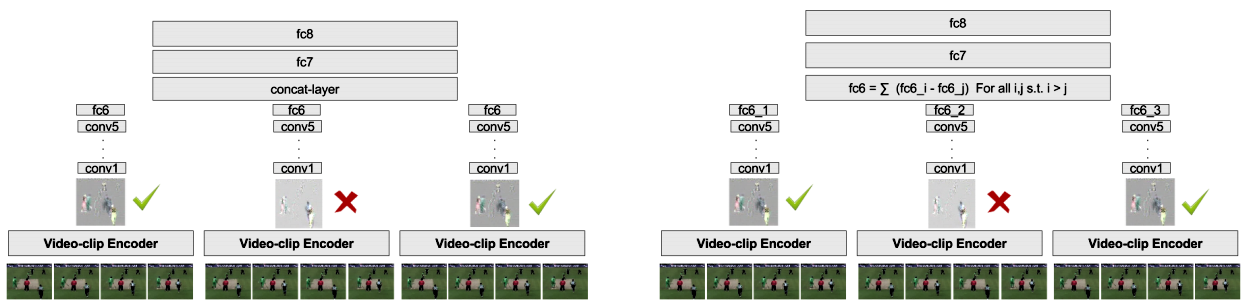
\includegraphics[width=\textwidth]{images/o3n1.png}
    \caption{Concatenation Model and Sum of Difference Model}
    \label{fig:fusionmodel}
\end{figure*}

Odd-one-out uses temporal ordering for representation learning in self supervised way.
This network is a new way to learn visual features for videos without using category level annotations. This method is applied to self supervised video representation learning where they sample sub sequences from videos and ask the network to learn to predict the odd video sequence. Here the odd video sub sequence is sampled such that it has wrong temporal order of frames while the even ones have the correct temporal order. 
They transfer weights to action recognition and fine tune on supervised set and show improvement over fully supervised learning.

Given $(N+1)$ number of sub sequenced videos from one single video, $N$ are in correct chronological order of frames which is the even set. The odd set consist of frame sampled from invalid sub sequenced video. One out of $(N+1)$ elements is odd object. Furthermore the position of the odd element is randomized by shuffling sequence permutation. Thus the odd one out prediction task reduces to an $(N+1)$ way classification problem, which can be solved by maximum likelihood estimation. The categorical cross-entropy loss is used for this after taking the softmax of the fc8 output as in standard $(N+1)$-way classification.
\begin{equation}
\lagr_O(x) = -\sum_n \sum_i y_i \log \hat{y}_i^{(n)}
\end{equation}
where $y_i$ denotes the label of the $i$-th frame and $\hat{y}_i^{(n)}$ denotes the predicted probability for the $i$-th frame for the $n$-th video in a batch.

To learn this, they use a  multibranch CNN consisting of $(N+1)$ input branches. Each branch contains 5 convolutional layers with a final fully connected layer. The branches are then fused and two more fully connected layer are used to produce the final result. The authors test two approaches for fusion,  concatenation, where the features are simply concatenated in order from each branch, and sum of difference where the difference between consecutive fc6 outputs are taken and the differences are summed. Their network architecture for both fusion techniques is shown in Figure \ref{fig:fusionmodel}.

Since the space of video frames is large and variable, the videos are sampled into fixed length sequences. The authors tested three different representations for the frames: sum of difference, stack of difference and dynamic images. Sum of difference works in the same way as the fusion layer, several consecutive frames are sampled and their difference taken. The result is summed to give a single image as input. Stack of difference again takes the difference between consecutive frames but this time the differences are encoded as separate channels in a multi-channel input.  Dynamic images are produced by smoothing the frame sequence using a moving average. The smoothed sequence is then transformed into a single image using the sum of difference method. The authors find that the stack of difference method performs the best, likely since it preserves the most information, so it is the only representation we test in this work. 
